I förra kapitlet togs en differentialekvation fram som beskriver vårat system som en relation mellan insignalen och utsignalen. Utifrån denna differentialekvation kan nu olika systemegenskaper tas fram som gör det möjligt att analysera systemet. Systemet kommer regera olika beroende på systemparametrarna, exempelvis kommer linan svänga olika beroende på vikten av personen på linan.

Systemanalysen kommer titta närmare på följande funktioner: systemfunktionen, impulssvaret, stegsvaret, rampsvaret, frekvensfunktionen samt amplitud- och faskaraktäristiken.
Vissa av dessa funktioner tas fram med hjälp av olika transformer som existerar i frekvensdomänen vilket kommer diskuteras i nästa kapitel.

\textbf{(ny sida här för att få figuren på nästa sida att komma på rätt ställe, kanske går att fixa senare)}
\newpage
\subsection{Frekvensdomänen}
\textbf{Vill gärna ha ett eget kapitel om detta eftersom det är väldigt viktigt att förstå när det gäller (linjära) system. Det kanske egentligen säger emot lite att man inte ska en separat inledande teoridel. Vad tycker ni?}

Tidigare i rapporten har vi sett på insignalen och utsignalen som funktioner av tid. Vi kommer nu behöva betrakta hur signalerna beter sig i frekvensdomänen där man istället kollar på vilka frekvenser som signal är uppbyggd av.

Till exempel kan signalen $x(t) = 3sin(2t) + sin(4t)$ ses som summan av två amplituder i tidsdomänen. I frekvensdoämen skulle den dock vara uppdelad i dess frekvenskomponenter, i detta fall två stycken vid frekvenserna $2$ och $4$.

\begin{figure}[h] % h = here
    \centering
    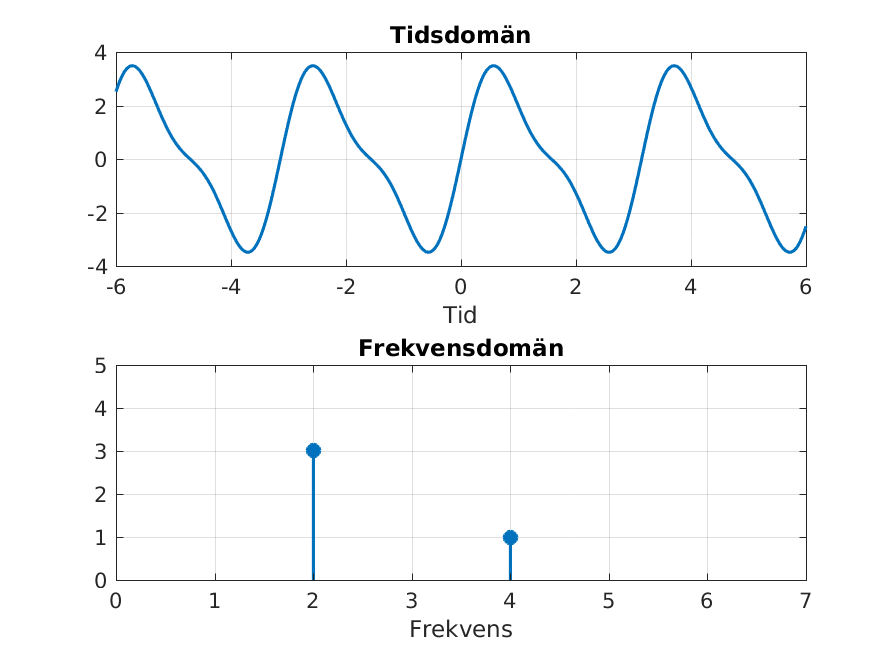
\includegraphics{bilder/tid_vs_frekvens_exempel}
    \caption{Tidsdoämen och frekvensdomänen för signalen $x(t)=3sin(2t)+sin(4t)$}
    \label{fig:tid_vs_frekvens_exempel}
\end{figure}

För systemanalysen kommer transformer som överför funktioner från tidsdomänen till frekvsensdomänen att användas, speciellt Laplacetransformen och Fouriertransformen.
Laplacetransformen är ett vanligt verktyg för att lösa differentialekvationer. För att ta sig tillbaka till tidsdomänen från frekvensdomänen kan inverstransformer appliceras.

\subsection{Systemfunktion}
\textbf{Ordningen på vissa meningar kanske borde ändras här så vi tar upp saker precis då vi behöver dom. Viktigast är att vi har en logisk följd av de vi försöker säga.}

Systemfunktionen beskriver ett förhållande mellan utsignalen och insignalen i frekvensdoämnen. Detta betyder att man kan räkna ut en utsignal om man vet insignalen i frekvensdoämnen och systemfunktionen. 
Detta går också att göra i tidsdomänen med faltning men det är oftast enklare att utföra beräkningen i frekvensdoämen.

För att beräkna systemfunktionen kommer hela differentialekvationen för systemet att Laplacetransformeras till frekvensdomänen. Det finns två versioner av Laplacetransformen som kan användas: den enkelsidiga och den dubbelsidiga.
Eftersom .

(alltså att en utsignal inte beror på tidigare händerlser i system) Detta brukar kallas att system är kausault.
Den enkelsidiga Laplacetransformen för en funktion $x(t)$ definieras som:

$$X(s) = \mathcal{L}\big\{x(t)\big\} = \int\limits_{0-}^{\infty} x(t)e^{-st}\,dt$$

där s är en komplexvärd frekvens.
Här används versaler för att beteckna funktioner i frekvensdomänen.
Denna transform behöver inte vara definierad för alla $s$ utan kan divergera i vissa fall. Därför är det viktigt att säga vart den transformerade funktionen är definierad. 



i denna rapport kommer en tabellen \textbf{NAMN} användas för att beräkna Laplacetransformerna.

Laplaca båda sidor (här får vi även massor av y(0-) termer som kommer försvinna pga kausalitet, NÄMN DETTA.

Bryt ut Y(s), ta fram H(s).

$$$$

\subsection{Impulssvar}


\subsection{Stegsvar}


\subsection{Rampsvar}
Är detta relevant? 

\subsection{Frekvensfunktion}


\subsection{Amplitud- och faskaraktäristik}


\subsection{Utsignal}
